%version of 07-0-19

\chapter{Graphs II:
Graphs within Computation and Communication}
\label{ch:Graphs2}
\index{graph}

Graphs provide one of the richest technical and conceptual frameworks
in the world of computing.  They provide concrete representations of
manifold data structures that should be studied in depth
in preparation for a ``Data Structures and Algorithms'' course.  They
embody tangible abstractions of relationships of all sorts, hence must
be well understood in order to discuss entities as varied as
web-search engines and social networks with precision and rigor.  As
with most of the topics we discuss in this text, graph-oriented
concepts must be taught ``in layers''.  All students should be
conversant with the use of graphs to represent and reason about a vast
array of complicated relationships---ranging from taxonomies
(including intra-family structures) to link-based data structures to
interconnectivity within social media, and on and on---but the degree
of sophistication that an individual student requires depends both on
the abilities of the student and the range of graph-modeled concepts
that will appear in the student's program.  The most-basic concepts in
this chapter should be understood by all students in any academic
program that includes a computation-oriented component---although each
concept can be developed with more texture and nuance within the
context of specific application domains; the more advanced concepts
should be selected with care, based on the instructor's perception of
students' needs, in the light of the ever-growing importance of
concepts involving interconnectivity.

Many developments in computing technology over recent decades have
made it imperative that graphs no longer be viewed by students as the
static objects introduced early in the history of computational
studies.  For instance, while it was innovative in the 1960s to employ
graphs and trees computationally as abstractions of data structures, such a view
is standard today.  Similar remarks, perhaps with differing dates, can
be made about graphs as vehicles for representing the flow of control
and information and as vehicles for representing interconnectivity
among both concepts and populations.  Applications ranging from
databases to web-search engines to social networks demand an
appreciation of graphs as dynamic objects.  This change in perspective
affects many aspects of the mathematical prerequisites for any
academic program that includes a computation-oriented component.

%%%%%%%%%%%%%%%%%%%%%%%%%%%%%

\section{Graph Coloring and Chromatic number}
\label{sec:graph-color}
\index{graph!node-coloring}

This section introduces the notion of {\it graph coloring}, and its
associated notion of the {\it chromatic number}
\index{graph!chromatic number} of a graph.

A {\it node-coloring} \index{graph!node-coloring} of a graph $\g$ is
an assignment of labels to $\g$'s nodes, in such a way that all of a
node $v$'s neighbors get a different label than $v$.  Traditionally,
the labels are called {\it colors}, for that term's evocative power.
The {\it chromatic number} \index{graph!chromatic number} of a graph
$\g$ is the smallest number of colors that can be used in a legal
node-coloring of $\g$.  In traditional parlance, the assertions

``$\g$ has chromatic number $c$'' \ \ \ \ \ and \ \ \ \ \
``$\g$ is {\it $c$-colorable}''
\index{graph!$c$-colorable}

\noindent
are considered to be synonymous.

{\Denis I added the following remark, do you agree?}
This notion is an important characteristic of a graph.
It is like an intermediate concept between the degree (local)
and diameter (global), which are easy to compute. 
The chromatic number is not easy to compute.
\bigskip

\noindent \fbox{
\begin{minipage}{0.95\textwidth}
The notion of graph coloring can be used to computational advantage to
model a broad variety of situations.  An extremely important, and
illustrative, use of graph coloring is to model {\it distributed}
computing.  In this setting, the nodes of a computation-graph $\g$
represent {\it agents}, such as, e.g., processing elements in a
computer; and $g$'s edges represent {\it communication links} that
enable each node $u$ to check its neighbors' states before any action
and to inform its neighbors of state-changes occasioned by an action
of $u$.  
%{\Denis actually, coloring is useful in any situation to express incompatibility between items}
The prohibition against ``monochrome'' edges---i.e., edges
both of whose incident nodes have the same color---guarantees that
node $u$ and all of its like-colored nodes can act at the same instant
with no fear of missing an important input to those actions.  Indeed,
one often encounters programs for distributed computing that look
something like

1. All {\em red} nodes perform an action

2. All {\em green} nodes perform an action

3. All {\em blue} nodes perform an action

\hspace*{1in} $\vdots$
\end{minipage}
}

\bigskip

Most of the ``named'' graphs in
Section~\ref{sec:graphs-important-families} have very small chromatic
numbers.  This is no accident: These graphs were invented (or, at
least, placed in the spotlight) because of their importance to the
topic of parallel and distributed computing---and we suggested only a
few paragraphs ago how to use graph node-colors to orchestrate some
such computations.  Accordingly, we devote this section to studying
graphs with very small chromatic numbers.

\subsection{Graphs with chromatic number $2$}
\label{sec:2-color-graphs}

We begin to garner intuition about graph coloring by exposing a large
set of graphs with chromatic number $2$.  In fact, we can completely
characterize these graphs structurally.

A graph $\g$ is {\it leveled} \index{graph!leveled} if there exists
an assignment of {\it level numbers} $\{ 1, 2, \ldots, \lambda\}$ to the
nodes of $\g$ in such a way that every neighbor of a level-$\ell$ node
$u$ resides either on level $\ell +1$ or on level $\ell -1$.

\begin{prop}
\label{thm:leveled=2-color}
A graph $\g$ has chromatic number $2$ if, and only if, it is leveled.
\end{prop}

\begin{proof}
Say first that $\g$ is a leveled graph.  Then labeling each node of
$\g$ with the (odd-even) parity of its level provides a valid
$2$-coloring of $\g$.

Say next that $\g$ is $2$-colorable.  Pick any node $v$ of $\g$ and
assign it to be the unique node on level $1$.  Let all neighbors of
$v$ be assigned to level $2$.  Continuing iteratively, say that the
largest level-number that we have employed---i.e., assigned nodes
to---is $\ell$.  Then we now assign to level $\ell +1$ all neighbors
of level-$\ell$ nodes which have not yet been assigned to a level of
$\g$.  Because $\g$ is $2$-colorable, each of the levels we have
specified is monochromatic, so that each edge of $\g$ connects a node
of one color with a node of the other color.  \qed
\end{proof}

We can now show that the following named graphs are $2$-colorable.

\begin{corol}
\label{thm:list-2-colorables}
The following graphs are leveled, hence have chromatic number $2$.

{\bf (a)}
any tree (which includes any path-graph $\p_n$)
{\Denis check here is path graph has well been defined before... Or include a reference}

{\bf (b)}
any cycle-graph $\cc_n$ that has an even number $n$ of nodes

{\bf (c)}
any mesh-graph $\m_{m,n}$

{\bf (d)}
any torus-graph $\widetilde{\m}_{m,n}$ that has an even number of
diagonals, i.e., even $m+n$

{\bf (e)}
any hypercube $\q_n$
\end{corol}

\begin{proof}
We provide a detailed sketch for each of the five graph families in
turn.

\noindent {\bf (a)}
We follow the procedure from the second half of the proof of
Proposition~\ref{thm:leveled=2-color} to expose a level structure in
any tree $\t$, as follows.  Pick any node $v$ of $\t$ and make it the
unique node on level $1$.  Let all neighbors of $v$ be assigned to
level $2$.  Continuing iteratively, say that the largest level-number
that we have employed is $\ell$.  Then we now assign to level $\ell
+1$ all neighbors of level-$\ell$ nodes which have not yet been
assigned to a level of $\t$.

Of course this process can be simplified when $\t$ is a path-graph
$\p$, by choosing one of $\p$'s end-nodes as node $v$.  We thereby
have precisely one node on each level, whereas the general procedure
can have levels with $2$ nodes.  A lesson here is that {\em a graph
  may admit many distinct level structures}.

\medskip

\noindent {\bf (b)}
When we apply the procedure of part (a) to an even-length cycle
$\cc_{2n}$, we produce a level structure in which levels $1$ and $n+1$
have one node apiece, while all other levels have two nodes apiece.

\medskip

\noindent {\bf (c)}
The edge-structure of mesh-graphs ensures that the labeling of each
node $\langle i,j \rangle$ of $\m_{m,n}$ with the odd-even parity of
the number $i+j$ is a $2$-coloring of $\m_{m,n}$.

\medskip

\noindent {\bf (d)}
The labeling in part (d) provides a $2$-coloring of any torus-graph
$\widetilde{\m}_{m,n}$ with even $m+n$.

\medskip

\noindent {\bf (e)}
Each edge of a hypercube $\q_n$ connects a node $v = \beta_1 \beta_2
\cdots \beta_n$, where each $\beta_i \in \{0,1\}$, to a node $v' =
\beta'_1 \beta'_2 \cdots \beta'_n$ where precisely one $\beta_j$
differs from $\beta'_j$.  Therefore, the following aggregation of
nodes of $\q_n$ into sets $S_0, S_1, \ldots, S_n$ provides a valid
leveling of $\q_n$.

Assign node $v = \beta_1 \beta_2 \cdots \beta_n$ to set $S_k$
precisely if $k$ of the bits $\beta_i$ equal $1$.
\qed
\end{proof}

The reader can show that no odd-length cycle $\cc_{2n+1}$ with $n \geq
1$ is $2$-colorable.  In like fashion, no graph $\g$ that {\em
  contains} an odd-length cycle can be $2$-colored.  This is the
problem that plagues the torus $\widetilde{\m}_{m,n}$ when $m+n$ is
odd.
\ignore{  {\Arny Put the odd cycle and torus as Exercises}}

The existence of odd-length cycles prevents {\em every} de Bruijn
network $\d_n$ from being $2$-colorable.  As small examples, one
observes the $3$-cycle
\[ 00 \ \rightarrow \ 01 \ \rightarrow \ 10  \rightarrow \ 00 \]
in $\d_2$ in Fig.~\ref{fig:dB2by2} and the $3$-cycle
\[ 001 \ \rightarrow \ 010 \ \rightarrow \ 100 \ \rightarrow \ 001 \]
in $\d_3$ in Fig.~\ref{fig:dB2by3}.  In fact, these small odd-length
cycles are only the proverbial tip of the iceberg for de Bruijn
networks.  The following result asserts that de Bruijn networks are
{\it directed-pancyclic}, \index{graph!pancyclic} 
\index{de Bruijn network!pancyclicity} \index{de Bruijn graph!pancyclicity}
meaning that they contain (even directed!)~cycles of {\em all}
possible lengths, both odd and even.  The proof of this result is
outside the scope of this text, but it should be accessible to the
motivated reader.

\begin{prop}{\cite{Yoeli62}}
For all $n$, the order-$n$ de Bruijn
network $\d_n$ is directed-pancylic, i.e., it
contains directed cycles of all possible lengths $1, 2, \ldots, 2^n$.
\end{prop}

\subsection{Planar and Outerplanar Graphs}
\label{sec:planar+outerplanar-color}
\index{planar graphs}
\index{outerplanar graphs}
\index{graph!planar}
\index{graph!outerplanar}

In this section, we focus on two graph families that are defined in
terms of the way they can be drawn (on a two-dimensional medium, such
as a piece of paper).
\bigskip

\noindent \fbox{
\begin{minipage}{0.95\textwidth}
The reader should not view this attention to how a graph can be drawn
as just an abstract game.  The process of designing and implementing
circuits within the constraints of {\it VLSI}, \index{VLSI} {\it Very
  Large Scale Integrated Circuit} technology,
\index{Very Large Scale Integrated Circuit technology}
\index{VLSI:Very Large Scale
Integrated Circuit technology} are very similar to drawing a circuit
on a two-dimensional medium.  We refer the reader to the revolutionary
1979 text \cite{Mead-Conway} for an introduction to this fascinating
technology, which requires technical literacy but little specialized
knowledge.
\end{minipage}
}
\bigskip

\noindent
A graph is {\it planar} \index{graph!planar} \index{planar graphs}
precisely if it can be drawn {\em without any crossing edges}.  A
graph $\g$ is {\it outerplanar} \index{graph!outerplanar}
\index{outerplanar graphs} precisely if it can drawn by {\em placing
  its nodes along a circle in such a way that its edges can be drawn
  as noncrossing chords of the circle}.  The latter condition is
equivalent to demanding that $\g$'s edges can be drawn within the
circle without any crossings.

We urge the reader to garner intuition about the graphs in these
families by experimenting with drawing some specific, rather complex
graphs.
\begin{itemize}
\item
The first set of graphs to draw are cliques, as defined in
Section~\ref{sec:clique}.  The cliques $\k_3$, $\k_4$, and
$\k_5$ will help expose the nature of the planar and outerplanar
graphs, because:
  \begin{itemize}
  \item
$\k_3$ is outerplanar; 
  \item
$\k_4$ is planar but not outerplanar;
  \item
$\k_5$ is not planar.
  \end{itemize}

\item
The ``bipartite'' cousins of the cliques will also yield valuable
insights.  For postive integers $m$ and $n$, the $m \times n$
bipartite clique $\k_{m,n}$ \index{bipartite clique} is the graph
whose node-set comprises the ordered pairs of integers:
\[  \n_{\fk_{m,n}} \ = \
\{ \langle i,j \rangle \ \ | \ \ 1 \leq i \leq m; \ \ 1 \leq j \leq n\}
\]
and whose edges connect each node $\langle i,j \rangle$ to every node
$\langle i,k \rangle$ with $1 \leq k \leq n$ and to every node
$\langle h,j \rangle$ with $1 \leq h \leq m$.

The second set of graphs to draw are the bipartite cliques $\k_{1,3}$,
$\k_{2,3}$, and $\k_{3,3}$.  These graphs will also help expose the
nature of the planar and outerplanar graphs, because:
  \begin{itemize}
  \item
$\k_{1,3}$ is outerplanar; 
  \item
$\k_{2,3}$ is planar but not outerplanar;
  \item
$\k_{3,3}$ is not planar.
  \end{itemize}
\end{itemize}

We selected the preceding cliques and bipartite cliques to ``play
with'' very carefully.  Using arguments that go beyond the scope of
this text, one can prove the following {\em characterization via
  exclusion} result, which characterizes each of our graph families by
identifying {\it forbidden subgraphs}.  \index{forbidden subgraphs}
\index{forbidden subgraphs!characterization of planar graphs}
\index{forbidden subgraphs!characterization of outerplanar graphs} The
notion of {\it graph homeomorphism} plays a fundamental role in
\index{graph!homeomorphism} the characterization.  This is a
dauntingly named technical term that is easily understood informally.
A {\it homeomorph} \index{graph!homeomorph} of a graph $\g$ is
obtained by adding (degree-$2$) nodes along one or more edges of $\g$.
The characterization of planar graphs by exclusion resides in a
celebrated theorem by the Polish mathematician and logician Kazimierz
Kuratowski; \index{Kuratowski, Kazimierz} the analogous result for
outerplanar graphs was derived by the French mathematician Gary
Chartrand \index{Chartrand, Gary} and the American mathematician Frank
Harary. \index{Harary, Frank}

\begin{theorem}
\label{thm:planar+outerplanar-exclusion}
{\bf (a)} {\rm \cite{ChartrandB67}}
A graph is outerplanar if, and only if, it does not have a subgraph
that is homeomorphic to either $\k_4$ or $\k_{2,3}$.

{\bf (b)} {\rm \cite{Kuratowski30}}
A graph is planar if, and only if, it does not have a subgraph
that is homeomorphic to either $\k_5$ or $\k_{3,3}$.
\end{theorem}


\subsubsection{Outerplanar graphs}

We look first at the smaller of this section's graph families, namely,
the {\it outerplanar graphs}. \index{outerplanar graphs}
\index{graph!outerplanar} (We shall remark in the following subsection B why these
graphs are called {\em outer}-planar.)

We begin our discussion of outerplanar graphs with some basic facts
about the family.

\begin{prop}
Every tree is outerplanar.
\end{prop}

We leave to the reader the challenge of proving this property. 
As an help, Fig.~\ref{fig:treeoutplanar} shows the way to distribute the nodes along a circle for the graph of Fig.~\ref{fig:tree}.

\begin{figure}[hbt]
\begin{center}
       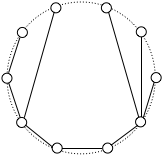
\includegraphics[scale=0.5]{FiguresGraph/TreeOutplanar}
       \caption{Outerplanar representation of the tree of Fig~\ref{fig:tree}.}
  \label{fig:treeoutplanar}
\end{center}
\end{figure}

\ignore{
We leave to the reader the challenge of drawing a tree in a way that
exposes its outerplanarity.  
{\Arny Another exercise}
}

\begin{prop}
\label{thm:basic-outerplanar-stuff}
Let $\g$ be an outerplanar graph.  Then:

\begin{tabular}{ll}
{\bf (a)} &
$\g$ is planar. \\
\ignore{{\bf (b)} &
$\g$ is a subgraph of a Hamiltonian graph. 
{\Denis I removed the second item since Hamiltonian has been shifted after this section.}\\}
{\bf (b)} &
Every subgraph of $\g$ is outerplanar. \\
{\bf (c)} &
At least one of $\g$'s nodes has degree $\leq 2$.
\end{tabular}
\end{prop}

\begin{proof}
{\bf (a)} $\g$'s planarity can be inferred from the ability to draw
$\g$'s edges as noncrossing chords of the circle.

\medskip
\ignore{
\noindent {\bf (b)} $\g$'s ``sub-Hamiltonianicity'' can be inferred
from the ability to draw $\g$ with its nodes along a circle.

\medskip}

\noindent {\bf (b)} We can produce an outerplanarity-witnessing
drawing of any subgraph of $\g$ by erasing some nodes and/or some
edges from our outerplanarity-witnessing drawing of $\g$.

\medskip

\noindent {\bf (c)} One verifies easily that this result holds for all
outerplanar graphs having $3$ or fewer nodes.  Focus, therefore, on an
arbitrary outerplanar graph $\g$ that has more than $3$ nodes.  Since
adding more edges to a graph cannot decrease the degree of any node,
we lose no generality by focusing on a graph $\g$ that is {\em maximal}
outerplanar, \index{maximal outerplanar graph} in the sense that
adding any new edge to $\g$ would destroy its outerplanarity.

Because $\g$ has more than $3$ nodes, and because all of its nodes lie
on a circle (in the drawing that witnesses its outerplanarity), there
must be pairs of nodes of $\g$ that are not adjacent along the circle.
Let $u$ and $v$ be nonadjacent nodes such that the distance between
$u$ and $v$ (measured in term of number of edges that must be traversed to reach one
from the other) is minimal among pairs of nodes nonadjacent nodes.  We
consider two cases.
\begin{itemize}
\item
If the distance between $u$ and $v$ were $2$, then the unique node
that lies between $u$ and $v$ along the circle would have degree $2$.
\item
If, on the other hand, the distance between $u$ and $v$ {\em exceeded}
$2$, then there would be at least {\em two} nodes that lie between $u$
and $v$ in either direction around the circle.  But in this case,
there would be two nonadjacent nodes that were closer to one another
than $u$ and $v$---which contradicts our choice of $u$ and $v$ as a
pair of closest nonadjacent nodes.
\end{itemize}
We conclude that $\g$ must have a node of degree $\leq 2$, completing
the proof.
\qed
\end{proof}

\bigskip

Our primary concern in this section is, of course, on graph coloring.
We return to this topic now.  The $3$-node cycle $\cc_3$ witnesses the
fact that not every outerplanar graph is $2$-colorable; $3$ colors is
the best that we can hope for.  We now show that this hope can be
realized.  The inductive proof of the following result can easily be
turned into an efficient node-coloring algorithm for outerplanar
graphs.

\begin{prop}[The $3$-Color Theorem for Outerplanar Graphs]
\label{thm:OP-3-colorability}
Every outerplanar graph is $3$-colorable.
\end{prop}

\begin{proof}
We proceed by induction on the number of nodes in the outerplanar
graph to be colored.

The base cases of the result are provided by small outerplanar
graphs---say those having $3$ nodes or fewer.

We assume, for induction, that every outerplanar graph having fewer
than $n$ nodes is $3$-colorable.

Let us now focus on an arbitrary $n$-node outerplanar graph $\g$.  By
Proposition~\ref{thm:basic-outerplanar-stuff}(d), $\g$ has a node $v$
of degree $\leq 2$.  Let us remove node $v$ from $\g$, along with the
edge(s) that connect $v$ to the rest of $\g$; call the resulting graph
$\g'$.  Now, $\g'$ is clearly outerplanar, once we ``stitch'' together
the circle we ``damaged'' by removing $v$, and $\g'$ has fewer than
$n$ nodes.  By induction, therefore, $\g$ is $3$-colorable.  But now
we can reattach node $v$ to $\g'$ by replacing the edges that attach
$v$ to $\g$.  Moreover, we can now color $v$ using whichever of the
$3$ colors on $\g$ that is {\em not} used for $v$'s neighbors in $\g$.
We have, thus, specified a $3$-coloring of $\g$, which extends the
induction and completes the proof.  \qed
\end{proof}

\ignore{**************
Two remarks about Proposition~\ref{thm:OP-3-colorability}:
\begin{enumerate}
\item
Our proof of the proposition can easily be transformed into an
algorithm that $3$ colors any $n$-node outerplanar graph in a
number of inductive stages that is a low-degree polynomial in $n$.
\item
The color-bound of the proposition can, of course, not be improved, as
witnessed by odd-length cycle-graphs.
\end{enumerate}
*************}


\subsubsection{Planar graphs}

The larger of this section's two graph families comprises {\it planar
  graphs} \index{planar graphs} \index{graph!planar} i.e., graphs
that can be drawn (on a two-dimensional medium, such as a piece of
paper) with no crossing edges.  The original focus on planar graphs
stemmed from viewing them as abstractions of geographical maps.

The $4$-node clique $\k_4$ witnesses the fact that not every planar
graph is $3$-colorable.  To wit, because every pair of nodes of every
clique are neighbors of each other, it follows that:

\smallskip

{\em For all $n$, the $n$-node clique $\k_n$ can be colored with $n$
  colors but no fewer.}.

\smallskip

\noindent
A century-plus attempt to prove that $4$ colors suffice for planar
graphs culminated in one of the most fascinating dramas in modern
mathematics, as American mathematicians Kenneth Appel 
\index{Appel, Kenneth}
and Wolfgang Haken, \index{Haken, Wolfgang}---with the help of their
families and of their computer!---announced their two-article-long
proof in 1974 of their renowned {\it $4$-Color Theorem for Planar
  Graphs}.  \index{The $4$-Color Theorem for Planar Graphs}
\index{coloring planar graphs!the $4$-Color Theorem}

\begin{theorem}[The $4$-Color Theorem for Planar Graphs~\cite{AppelH77a,AppelH77b}]
\label{thm:Four-ColorTheorem}
Every planar graph is $4$-colorable.
\end{theorem}

The proof of Theorem~\ref{thm:Four-ColorTheorem} is beyond the scope
of any introductory text, but the backstory of the proof is truly
fascinating---and it supplies ample motivation for the proofs of the
$6$-color and $5$-color analogues of the Theorem.  Beginning with a
failed attempt, in 1875, to prove that every planar map can be colored
with four colors with no abutting countries getting the same color,
the so-called {\it $4$-Color Problem}
\index{The $4$-Color Problem for planar graphs} 
held the world of discrete mathematics in thrall for roughly a century
before But the drama surrounding the $4$-Color Problem persisted,
because of the Appel-Haken proof's reliance, in a fundamental way, on
a computer program that checked more than a thousand essential---but
clerical---assertions (about forbidden subgraphs).  It took the
mathematics community years before this proof, with its massive
complexity and unprecedented employment of ``collaboration'' by
computer, was generally accepted.  In addition to the primary
references \cite{AppelH77a,AppelH77b} that accompany our statement of
the Theorem, we recommend to the interested reader the articles
\cite{AppelH77c,AppelH89} that summarize and, at a rather
sophisticated level, popularize this marvelous mathematical tale.

We turn now to the $6$-color and $5$-color analogues of the $4$-color
Theorem.  The weaker, $6$-color, version of the Theorem can be proved
in much the same way as its outerplanar-graph cousin,
Proposition~\ref{thm:OP-3-colorability}.  The proof of the stronger,
$5$-color, version of the Theorem already requires us to break the
world into multiple cases---but only a single-digit number of cases,
in contrast to the four-digit case list one encounters with the proof
of Theorem~\ref{thm:Four-ColorTheorem} \cite{AppelH77a,AppelH77b}.

\bigskip

{\it The $6$-Color Theorem for Planar Graphs.}
The first step in showing that every planar graph can be colored using
$6$ colors resides in the following analogue for planar graphs of
Proposition~\ref{thm:basic-outerplanar-stuff}(d), which asserts that
every outerplanar graph has a node of degree $2$.

\begin{lemma}
\label{thm:PlanarGraph-degree5}
Every planar graph has a node of degree $\leq 5$.
\end{lemma}

\begin{proof} {\em (Lemma~\ref{thm:PlanarGraph-degree5})}
Let us focus on a planar drawing of a (perforce) planar graph $\g$,
which has $n$ nodes, $e$ edges, and $f$ {\it faces}.  A {\it face}
\index{graph!planar!face in a drawing}
\index{planar graph!face in a drawing} 
in a drawing of $\g$ is a polygon whose sides are edges of
$\g$, whose points are nodes of $\g$, and whose interiors are empty,
in that no edge of $\g$ crosses through the interior.
\bigskip

\noindent \fbox{
\begin{minipage}{0.95\textwidth}
Now that we know about faces, we can finally describe the origin of
the term {\it outerplanar}.  A graph $\g$ is outerplanar if it can be
drawn with all of its nodes around a single ``outer'' face in such a
way that all of its edges are drawn in a noncrossing manner within the
``outer'' face.  In fact, we usually draw $\g$ so that the ``outer''
face is literally outside the ``outer'' face.
\end{minipage}
}
\bigskip

The following auxiliary result derives a celebrated ``formula'' of
Euler.  \index{Euler, Leonhard} \index{Euler's Formula}

\begin{prop} [Euler's Formula for Planar Graphs]
\label{thm:Euler-Formula}
Given the indicated drawing of $\g$, we have
\begin{equation}
\label{eqn:Eulers-formula}
n \ - \ e \ + \ f \ \ = \ \ 2
\end{equation}
\end{prop}

\medskip

We defer proving Proposition~\ref{thm:Euler-Formula} so that we can
proceed with our ongoing proof of Lemma~\ref{thm:PlanarGraph-degree5}.
\ignore{{\Denis Attention here: the ref is not written correctly after the compilation}}
We devote Subsection C to two quite different proofs of Euler's
celebrated formula.

\medskip

As we approach the next step of the proof, we simplify the setting by
assuming henceforth that $\g$ is connected and that it is {\em
  maximal}, \index{graph!planar!maximal} in the sense that one cannot
add any new edge to the drawing without crossing an existing edge.
This step only strengthen's the Lemma's conclusion by apparently
making it more difficult to find a small-degree node.

With this assumption in place, we now adapt a pedagological tool from
\cite{Berge73}, in order to make the following counting argument
easier to follow.  We construct a {\em directed bipartite} graph {\bf
  G} which exposes certain features of $\g$'s structure.  On one side
of {\bf G} are the $f$ faces of $\g$; on the other side are $\g$'s $e$
edges.  {\bf G} contains an arc from each face of $\g$ to
each edge of $\g$ that forms a ``side'' of the polygonal
drawing of the face.  Because $\g$ is a maximal planar graph, we have:
\begin{itemize}
\item
Each face of $\g$ is a $3$-cycle, hence involves three nodes.
\item
Each edge of $\g$ touches two faces.
\item
Each edge of $\g$ touches two nodes.
\end{itemize}

Let us now put these facts together, and assume, for contradiction,
that every node of $\g$ had degree $\geq 6$.  We would then find that
\[
\left[ f \ \ \leq \ \ \frac{2}{3} e \right] \ \ \ \ \mbox{ and } \ \ \ \
\Big[ e \ \ \geq \ \ 3n \Big]
\]
Incorporating these two bounds into Euler's Formula
(\ref{eqn:Eulers-formula}), we arrive at the following contradiction.
\[ 2 \ \ = \ \ n \ - \ e \  + \ f
\ \ \leq \ \ \frac{1}{3} e \ - \ e \ + \ \frac{2}{3} e \ \ = \ \ 0
\]
This contradiction proves that every planar graph must have a node of
degree $\leq 5$.
 \qed-Lemma~\ref{thm:PlanarGraph-degree5}
\end{proof}

\medskip

We finally have the tools to color planar graphs using $6$ colors.
\index{The $6$-Color Theorem for Planar Graphs}
\index{coloring planar graphs!the $6$-Color Theorem}

\begin{prop}[The $6$-Color Theorem for Planar Graphs]
\label{thm:P-6-colorability}
Every planar graph is $6$-colorable.
\end{prop}

\begin{proof}
The $2$-Color Theorem for Outerplanar Graphs
(Proposition~\ref{thm:OP-3-colorability}) and this result follows via
almost-identical inductions on the number of nodes in the graph $\g$
that is being colored.  Both arguments:
\begin{enumerate}
\item
remark that the coloring goal can be met for small graphs

For outerplanar graphs, ``small'' means ``$3$ or fewer nodes''.  For
planar graphs, it means ``$4$ or fewer nodes''.

\item
remove from $\g$ a node $v$ of smallest degree $d_v$, together with
all its incident edges

For outerplanar graphs, we guarantee that $d_v \leq 2$
(Proposition~\ref{thm:basic-outerplanar-stuff}(d)).  For planar
graphs, we guarantee that $d_v \leq 5$
(Lemma~\ref{thm:PlanarGraph-degree5}).

\item
inductively color the nodes of the graph $\g'$ left after the removal
of $v$

For outerplanar graphs, we color $\g'$ with $\leq 3$ colors
(Proposition~\ref{thm:OP-3-colorability}).  For planar
graphs, we use an inductive assumption that $\g'$ can be colored with
$\leq 6$ colors. 

\item
reattach $v$ via its $d_v$ edges and then color $v$.

Note that the coloring guarantee in both
results---Proposition~\ref{thm:OP-3-colorability} for outerplanar
graphs and the current result for planar graphs---allows us to use
$d_v +1$ colors to color $\g$.  Because $v$ has degree $d_v$, it is a
neighbor of no more than $d_v$ nodes of $\g'$, so our access to $d_v
+1$ colors guarantees that we can successfully color $v$.
\end{enumerate}
The proofs of the $3$-colorability of outerplanar graphs and the
$6$-colorability of planar graphs thus differ only in the value of
$d_v$.  \qed
\end{proof}

\bigskip

{\it The $5$-Color Theorem for Planar Graphs.}
\index{The $5$-Color Theorem for Planar Graphs}
\index{coloring planar graphs!the $5$-Color Theorem}
We now prove that every planar graph can be colored using $5$ colors.
\bigskip

\noindent \fbox{
\begin{minipage}{0.95\textwidth}
The case analysis in the following proof is a bit more complex than in
most of the results in the text, but a methodical reading should make
the proof quite accessible.  Moreover, {\em roadmap} of the case
analysis is a valuable lesson in how mathematics is really done!  For
instance, the motivated reader will be able to recast the totally
positive proof we present into the form of a proof by contradiction.
The positive version should be more to the taste of a computationally
oriented reader---but both proofs are equally correct.
\end{minipage}
}
\bigskip

\begin{prop}[The $5$-Color Theorem for Planar Graphs \cite{Heawood90}]
\label{thm:5colors}
Every planar graph is $5$-colorable.
\end{prop}

\ignore{************************
The proof again (I mean like for 6 colors) is by recurrence but we add
here a contradiction argument:
Similarly, we focus on a node with degree 5 (at some points, we will
have to justify this)
This node (call it x) has 5 neighbors
The problem is when they are colored by the 5 colors, otherwise it is
colored by a missing one.
Let now label these 5 nodes from 1 to 5.
Consider the nodes 1 and 3, colored by two different colors and the
sub-graph composed of nodes with colors 1 and 3
If these two nodes are in disjoint connected components, (case 1), it is
easy to color x by reverting the colors 1 and 3 in one component
(see figure)
Thus, the problem is when there exists an alternate path (in term of
colors) between node 1 and node 3
in this case (case 2), consider nodes 2 and 4, using a similar process
as in case 1, if there are two connected components
we are done (x can be colored by reverting the colors along the path
in one component), otherwise, there is an alternate path
between 2 and 4.
However, since the graph is planar, then, both alternate paths will
intersect, which is impossible
************************}


The proof is rather technical and is therefore relegated to the
Appendix, specifically as Chapter~\ref{Appendix:5colors}.


\ignore{***********
\begin{proof}
For brevity, let us henceforth discuss only {\em valid} colorings,
i.e., colorings of a graph's nodes in which neighboring nodes get
different colors.

\smallskip

\noindent {\em Base of our induction.}
Because the $5$-clique $\k_5$ is obviously $5$-colorable, so also must
be all graphs having $\leq 5$ nodes.  Therefore, we know that any
non-$5$-colorable graph would have $\geq 6$ nodes.

\smallskip

\noindent {\em Inductive hypothesis.}
Assume, for induction, that every planar graph having $\leq n$ nodes
is $5$-colorable.

\smallskip

\noindent {\em Inductive extension.}
If the proposition were false, then there would exist a planar graph
$\g$ having $n+1$ nodes which is not $5$-colorable.  By
Lemma~\ref{thm:PlanarGraph-degree5}, $\g$ would have a node $v$ of
degree $\leq 5$.  The remainder of the proof focuses on the graph
$\g$, its minimal-degree node $v$, and on $v$'s $(d_v \leq 5)$
neighbors in $\g$.

Now, if there were a coloring of $\g$'s nodes in which $\leq 4$ colors
were used to color $v$'s neighbors, then the following analogue of the
coloring strategy of Proposition~\ref{thm:P-6-colorability} would
produce a $5$-coloring of $\g$.
\begin{enumerate}
\item
Remove node $v$ and its incident edges from $\g$, thereby producing
the $n$-node planar graph $\g'$.
\item
Produce a $5$-coloring of $\g'$ that uses only $4$ colors for the
nodes that are neighbors of $v$ in $\g$.
\item
($a$) Reattach node $v$ and its edges to $\g'$, thereby reconstituting
  $\g$.  ($b$) Color $v$ with whichever of the $5$ available colors is
  not used to color $v$'s neighbors.
\end{enumerate}

In order to proceed in pursuit of a contradiction, we must understand
what structural features of $\g$ make it impossible to use only $4$
colors on $v$'s neighbors when $5$-coloring $\g$.  There are three
important situations to recognize.
\begin{description}
\item[{\sf Case 1}.]
Node $v$ has degree $\leq 4$.

\smallskip

By definition, $\leq 4$ colors are used to color $v$'s neighbors in
this case.
\end{description}
Note that, in all remaining cases, node $v$ has precisely $5$
neighbors---or else, we would have invoked Case 1 to color $\g$ with
$5$ colors.
\begin{description}
\item[{\sf Case 2}.]
For some $5$-coloring of $\g$, $\geq 2$ neighbors of $v$ get the same
color.

\smallskip

Because $v$ has exactly $5$ neighbors, in this case, only $4$ colors
are used to color these neighbors.
\end{description}
In all remaining cases, the $5$ neighbors of $v$ receive distinct
colors.
\begin{description}
\item[{\sf Case 3}.]
For some $5$-coloring of $\g$, some two neighbors of $v$, call them
$v_1$ and $v_2$, reside in distinct components of $\g$ once $v$ and
its incident edges are removed from $\g$.

\smallskip

As before, let $\g'$ be the (in this case, disconnected) graph that
results when $v$ and its incident edges are removed from $\g$.  For $i
= 1,2$ Let $\g_i$ be the component of $\g'$ that contains node $v_i$.

Say that, under the $5$-coloring of $\g$ that we are focusing on,
$v_1$ is colored {\it red} and $v_2$ is colored {\it green}.

Let us recolor the nodes of $\g_1$ so that node $v_1$ is now colored
{\it green}.  (One needs only switch the colors {\it red} and {\it
  green} in the existing coloring of $\g_1$.)  It is always possible
to do this in a way that does not affect the valid coloring of $\g_2$
because $\g_1$ and $\g_2$ are mutually disjoint.

Once we have thus-recolored $\g_1$, we have a $5$-coloring of $\g$ for
which Case 2 holds.  (In fact, we can color node $v$ {\em red} when we
reattach it to $\g'$.)
\end{description}

\noindent
We now see that Cases 1--3 cannot prevent us from $5$-coloring $\g$, so
we are left with the following minimally constrained situation.
\begin{description}
\item[{\sf Case 4}.]
\begin{itemize}
\item
Every minimum-degree node of $\g$ has $5$ neighbors.

For the minimum-degree node $v$, let us call these neighbors $v_1$,
$v_2$, $v_3$, $v_4$, $v_5$, in clockwise order within the planar
drawing.
\item
In every $5$-coloring of $\g$, the neighbors of every minimum-degree
node receive distinct colors.

For node $v$, let us say that neighbor $v_i$ receives color $c_i$.
\end{itemize}
The leftmost graph in FIGURE 1 
{Denis Put right ref here}
depicts the portion of $\g$ comprising
node $v$ and its neighbors.  In the figure, we use integer $i$ to
denote, ambiguously, node $v_i$ and its assigned color $c_i$.  The
question mark ``?'' that ``colors'' node $v$ indicates that we do not
yet know what color to assign to $v$.  The other two graphs in the
figure depict schematically how we have dealt with Case 3 above.
\begin{itemize}
\item
All neighbors of node $v$ remain in the same component of $\g$ when
$v$ and its incident edges are removed.
\end{itemize}
\end{description}
To analyze Case 4, we focus on nodes $v_1$ and $v_3$ in FIGURE 1.
{Denis Put right ref here}
Importantly, these nodes have received distinct colors ($c_1$ and $c_3
\neq c_1$, respectively), and these nodes are not adjacent to one
another as one makes a clockwise sweep around node $v$.

Now take $\g$ and focus only on the nodes that are colored $c_1$ or
$c_3$ (as are $v_1$ and $v_3$, respectively) and on the nodes that are
colored $c_2$ or $c_4$ (as are $v_2$ and $v_4$, respectively).  One
sees from Figure 2 that:
\begin{itemize}
\item
$\g$ can, {\em but need not}, contain a path whose nodes alternate
  colors $c_1$ and $c_3$---call this a ``$c_1$-$c_3$ path'' between
  nodes $v_1$ and $v_3$.
\item
$\g$ can, {\em but need not}, contain a path whose nodes alternate
  colors $c_2$ and $c_4$---call this a ``$c_2$-$c_4$ path'' between
  nodes $v_2$ and $v_4$.
\item
$\g$ {\em cannot} contain both of the paths just described, i.e., a
  $c_1$-$c_3$ path between $v_1$ and $v_3$ {\em and} a $c_2$-$c_4$ path
  between $v_2$ and $v_4$.

{\em These two paths, if they existed, would cross one another---which
  is forbidden because $\g$ is a {\em planar} graph.}  See Figure 2.
\end{itemize}
It follows that {\em either} $\g$ does not contain a $c_1$-$c_3$ path
between $v_1$ and $v_3$ {\em or} $\g$ does not contain a $c_2$-$c_4$
path between $v_2$ and $v_4$.  Say, with no loss of generality, that
the former path does not exist.  Then we can switch colors $c_1$ and
$c_3$ beginning with node $v_1$ and obtain a coloring of $\g$ in which
$v_1$ and $v_3$ both receive the color $c_3$.  We can then proceed as
in Case 2 to get a $5$-coloring of $\g$.

This four-case analysis shows that we can always produce a
$5$-coloring of $\g$, which completes the proof.  \qed
\end{proof}
}

We finish this topic with an overview of the intellectual
cost-benefit tradeoff we have observed:
\begin{itemize}
\item
A straightforward recursive coloring strategy suffices if one is
willing to settle for a six-color palette when coloring planar graphs
(Proposition~\ref{thm:P-6-colorability}).
\item
A four-case analysis, in which one case comprises multipl subcases, is
needed in order to eliminate one of the colors from the palette, to
achieve a five-color palette (Proposition~\ref{thm:5colors}).
\item
An analysis involving close to $2000$ cases is needed in order to
achieve the provable optimal, a four-color palette
(Theorem~\ref{thm:Four-ColorTheorem}).
\end{itemize}

\subsubsection{Two validations of Euler's Formula}
\index{Euler's Formula}

We develop two quite different proofs of
Proposition~\ref{thm:Euler-Formula}.

\medskip

\index{Euler's Formula!validation by structural induction}
\noindent {\bf Validatinging Euler's Formula by structural induction}.  We
validate (\ref{eqn:Eulers-formula}) by growing a planar graph $\g$
edge by edge.  We proceed by induction.

\smallskip

\noindent {\it Base case}.
The Formula clearly holds for the smallest planar graphs, including
the smallest interesting one, $\cc_3$, which has $n = e = 3$ and $f =2$
(the inner and outer faces of the ``triangle'').

\smallskip

\noindent {\it Extension}.
We grow the current version of $\g$ by adding a new edge.  Two cases
arise.
\begin{itemize}
\item
{\em The new edge connects existing nodes.}  In this case, this
augmentation of $\g$ increases the number of edges ($e$) and the
number of faces ($f$) by $1$ each, while keeping the number of nodes
($n$) unchanged.  Euler's Formula (\ref{eqn:Eulers-formula}) thus
continues to hold.

\item
{\em The new edge adds a new node, which is appended to some
  preexisting node.}  In this case, this augmentation of $\g$
increases the number of edges ($e$) and the number of nodes ($n$) by
$1$ each, while keeping the number of faces ($f$) unchanged.  Euler's
formula (\ref{eqn:Eulers-formula}) thus continues to hold.
\end{itemize}
This augmentation extends the induction, hence validates the Formula.
\qed

\bigskip

%{\Denis Here is a nice alternative proof for the Euler proposition}

\index{Euler's Formula!validation by deconstruction}
\noindent {\bf Validating Euler's Formula by deconstruction}.  Let us be
given a planar graph $\g$ that has $n$ nodes, $e$ edges, and $f$
faces.  We validate (\ref{eqn:Eulers-formula}) by deconstructing $\g$
and showing that each step in the process preserves as {\it invariant}
the expression $\phi(n,e,f) = n-e+f$.  \index{invariants}

\bigskip

\noindent \fbox{
\begin{minipage}{0.95\textwidth}
The concept of \textit{invariance} is an extremely important
conceptual tool when crafting proofs.  The underlying idea is to find
an expression $\phi(\cdot)$ whose value is preserved as a process
proceeds, step by step.  Rather than try to explain the concept in
abstraction, we recommend that the reader follow this proof of Euler's
Formula with an eye to keeping track of the invariant expression
$\phi(n,e,f)$ whose arguments are obtained from the subject planar
graph $\g$.
\end{minipage}
}
\bigskip

\noindent
We analyze the following two-phase process performed in sequence.
\begin{description}
\item[{\bf Phase 1}.]
Iterate the following process of removing edges from $\g$ until one
edge-removal reduces $\g$ to a graph with a single face.  This
termination condition is equivalent to stopping when the remaining
graph is a tree.  One can verify that the tree one ends up with is
{\em connected}.
\bigskip

{\bf The action}.
If the graph remaining at some step contains an edge that is shared by
two distinct faces, then remove any such edge.

Fig.~\ref{fig:planarStep1} illustrates the action of Step 1 for a
(residual) graph with $n=8$ nodes, $e=11$ edges, and $f=5$ faces.
\begin{figure}[hbt]
\begin{center}
   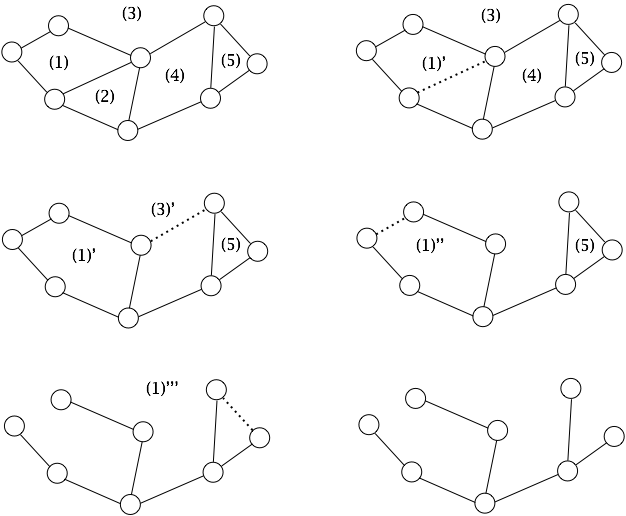
\includegraphics[scale=0.4]{FiguresGraph/planarStep1}
\caption{Illustrating Phase 1: From top left to bottom right, each
  transformation preserves the invariant $\phi(n,e,f)$.  The first
  transformation removes the edge shared by faces (1) and (2),
  creating a new, merged, face (1)'.}
  \label{fig:planarStep1}
\end{center}
\end{figure}

\bigskip

{\bf The analysis}.
\begin{itemize}
\item
The graph remaining after an edge-removal is still planar---edges are
removed but never added---so we can continue the process.
\item
The process preserves the value of function $\phi$.  To wit, $n$ is
unchanged, while $e$ and $f$ are each reduced by $1$: $\phi(n,e,f) =
\phi(n,e-1,f-1)$.
\end{itemize}

\item[{\bf Phase 2}.]
Iterate the following process of removing nodes from the tree produced
by Step 1, until only one node remains.
\bigskip

{\bf The action}.
Remove any leaf of the current tree, together with its incident edge.

Fig.~\ref{fig:planarStep2} illustrates the action of Step 2
for a tree  with $n=8$ nodes---hence, $e=7$ edges and $f=1$ face.
\begin{figure}[hbt]
\begin{center}
   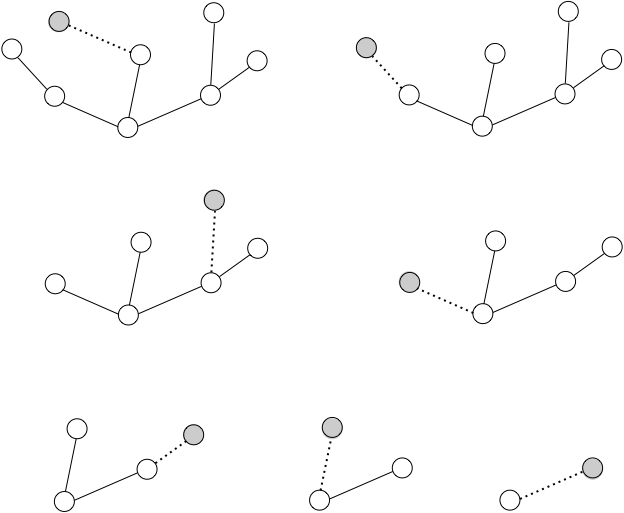
\includegraphics[scale=0.4]{FiguresGraph/planarStep2}
   \caption{Illustrating Phase 2: We remove a sequence of leaves, each
     with its incident edge, until we reach a single node.  Again,
     $\phi$ remains invariant after each leaf-removal.}
  \label{fig:planarStep2}
\end{center}
\end{figure}

\bigskip

{\bf The analysis}.
The value of function $\phi$ remains unchanged by each leaf-removal.
To wit, $f$ is unchanged (it remains at $1$), while $n$ and $e$ are
each reduced by $1$: $\phi(n,e,f) = \phi(n-1,e-1,f)$
\end{description}

\noindent {\bf The cumulative analysis}.
\begin{itemize}
\item
Our process executes a number of steps exactly equal to the number of
edges of the graph $\g$ that we began with.  To wit, the edge-removal
Step removes $e-n$ edges, while the leaf-removal Step removes $n$
nodes.
\item
At the end of the process, $e=0$ and $n=f=1$, so that the residual
value of $\phi$ is $2$.  Because each action prescribed by the process
preserved the value of $\phi$, we know that $\phi$ has the value $2$
before each edge-removal and leaf-removal.
\end{itemize}
We conclude that, at the
start of the process,  $\phi(n,e,f)$ had the value $2$.  In other
words, $n-e+f = 2$.  This concludes the proof.  \qed

\bigskip

\noindent \fbox{
\begin{minipage}{0.95\textwidth}

**ADD REFERENCES HERE

We presented several parameters for characterizing a graph.
The degree of the vertices (which is a local characteristic) 
and the diameter (which is a global characteristic).
Both parameters are easy to determine (done in polynomial time).
The chromatic number is an intermediate concept which provide a global information from local rules.
It is hard to compute for any graph. 

\cite{GareyJ79}
\cite{Karp72}

It is an {\sf NP}-complete problem to decide, given any fixed $k \geq
3$, whether a given graph $\g$ is $k$-colorable.

A simple argument shows that it is {\sf NP}-hard to find smallest
number of colors that provide a valid node-coloring of $\g$.

But one can exhibit ``greedy'' algorithms that give good results.
\end{minipage}
}


\section{Path and Cycle Discovery Problems in Graphs}
\label{sec:path-cycle-problems}

Just as various genres of {\it spanning trees} are used to
``summarize'' aspects of the connectivity structure of a connected
graph $\g$, various genres of {\it paths} and {\it cycles} in $\g$ are
often useful to ``summarize'' aspects of $\g$'s traversal structure.
This section is devoted to a range of problems related to determining
the existence in a graph $\g$ of a path or a cycle that {\em
  completely} ``summarizes'' $\g$'s traversal structure, either by
containing each node of $\g$ precisely once or by containing each edge
of $\g$ precisely once.  We shall generally focus in this section only
on {\em undirected} paths and cycles in {\em undirected}, {\em
  unweighted} graphs.  Extrapolating the notions we discuss to their
directed analogues in directed and/or weighted graphs, will be
accomplished via carefully crafted exercises.  In a similarly, but
simpler, vein, we shall generally discuss only prolems concerning {\em
  cycles}, leaving to the reader the analogous notions that concern
paths.  We begin by delimiting the two main classes of cycle-discovery
problems that we study in this section.

\smallskip

{\it Eulerian cycles (or, tours)}.  A cycle in a graph $\g$ that
traverses each of $\g$'s edges precisely once is called an {\it
  Eulerian cycle},\index{graph!Eulerian cycle} \index{Eulerian cycle}
(or, often, an {\it Eulerian circuit}).  \index{graph!Eulerian
  circuit} \index{Eulerian circuit} The edge-exhausting
cycles/circiuts/tours referred to by these several names were
introduced as a topic of study in 1736 by the Swiss mathematician
\index{Euler, Leonhard} Leonhard Euler, whose name we have already
encountered multiple times.  Euler allegedly discovered the topic
while contemplating how to design a tour of the town of K\"{o}nigsberg
that would cross each of the town's bridges precisely once.  The quest
for Eulerian cycles in graphs is, thus, one of the oldest problems in
the fields now called {\it Operations Research} and {\it graph
  theory}.  (An edge-exhausting {\em path} in $\g$ is referred to in
the obvious analogous way.)  When one views an Eulerian cycle as a
``map'' for traversing a graph---as did Euler when contemplating this
problem---one often calls the cycle an {\it Eulerian tour}.
\index{graph!Eulerian tour} \index{Eulerian tour} Traditionally, a
graph that admits an Eulerian cycle is said to be {\it
  Eulerian}. \index{graph!Eulerian} \index{Eulerian graph}

\medskip

Dually: A cycle in a graph $\g$ that encounters each of $\g$'s nodes
precisely once is called a {\it Hamiltonian cycle},
\index{graph!Hamiltonian cycle} \index{Hamiltonian cycle} (or, often,
a {\it Hamiltonian circuit}). \index{graph!Hamiltonian circuit}
\index{Hamiltonian circuit} This cycle-discovery problem is named in
honor of the British mathematician Sir William Rowan Hamilton,
\index{Hamilton, William Rowan} who is credited with inventing the
concept in the mid-19th century.  
{\Denis even if the problem was introduced some time before in its whole genericity by 
Thomas Penyngton Kirkman} (A node-exhausting {\em path} in
$\g$ is referred to in the obvious analogous way.)  When one views a
Hamiltonian cycle as a ``map'' for traversing a graph, one often calls
the cycle a {\it Hamiltonian tour}.  \index{graph!Hamiltonian tour}
\index{Hamiltonian tour} Traditionally, a graph that admits a
Hamiltonian cycle is said to be {\it
  Hamiltonian}. \index{graph!Hamiltonian} \index{Hamiltonian graph}

\medskip

Despite the conceptual duality between the edge-encountering goal that
underlies Eulerian paths and cycles, on the one hand, and the
node-encountering goal that underlies Hamiltonian paths and cycles,
these two graph-traversing goals differ in virtually every significant
respect.  It is rather easy to characterize the family of graphs that
admit Eulerian tours and to find such a tour if it exists
(Section~\ref{sec:EulerianCycle}); in contrast, there is no known
characterization of the family of graphs that admit Hamiltonian tours,
and the computational problem of efficiently determining whether a
graph admits such a tour is one of the major classical problems in the
field of computational complexity  (Section~\ref{sec:Hamiltonian-cycle}).

%%%%%%%%%%%%%%%%%%%%%%%%%%%%%%%%%%%%%%%%%%%%%%%%%%%%

\subsection{Eulerian Cycles and Paths}
\label{sec:EulerianCycle}

The main results in this section characterize the families of directed
and undirected graphs that admit an {\it Eulerian cycle} or an {\it
  Eulerian path}.  The proofs of these characterizations are
constructive: they consist of algorithms that efficiently find such a
cycle or such a path when one exists.  We focus on graphs that are
connected: the algorithms we present can actually be adapted to find
an {\it Eulerian cycle} or an {\it Eulerian path} in each connected
component of a general graph.  As we embark on our adventure, we note
that the problem of finding an Eulerian cycle in a graph $\g$ is
equivalent to the problem of drawing $\g$ without ever lifting one's
pencil. \index{graph!drawing without lifting pencil}

%\subsubsection{Characterizing Eulerian graphs, and finding Eulerian tours}
%\label{sec:eulerian-cycle-path}

There is a simple and elegant characterization of graphs that admit
Eulerian cycles and paths, which is accompanied by a simple and
efficent algorithm for testing a given graph for finding such a tour
in a graph that admits one.  We encapsulate four versions of the
desired result in the following statement.

\begin{prop}[Eulerian Cycles]
\label{thm:eulerian-cycle}
{\bf (a)}
An undirected graph $\g$ admits an Eulerian cycle if, and only if,
$\g$ is connected and every node of $\g$ has even degree.

{\bf (b)}
A directed graph $\h$ admits a directed Eulerian cycle if, and only if,
$\h$ is connected and, for every node $v$ of $\g$,
$\mbox{\sc indegree}(v) \ = \ \mbox{\sc outdegree}(v)$.
\end{prop}

\begin{proof}
The {\em necessity} of the conditions in both parts {\bf (a)} and {\bf
  (b)} is established by the two following observations.
\begin{itemize}
\item
By definition, a graph that is not connected does not admit any \textit{eulerian} cycle.
\item
Each cycle that a graph admits accounts for two edges per node,
because the cycle must ``enter'' the node by one edge and ``exit'' the
node by a different edge.
\end{itemize}

\smallskip

\noindent
We turn now to the verification of the {\em sufficiency} of the
Proposition's conditions.  Our argument resides in the following
``streamlined'' version of an induction---this is closer to the form
of an induction that one would encounter in practice, rather than in a
textbook.

The base case of the induction resides in proving the sufficiency of
the Proposition's conditions for ``small'' graphs.  
\bigskip

\noindent \fbox{
\begin{minipage}{0.95\textwidth}
While we largely
leave this step to the reader, we do want to discuss the definition of
``small''.  Until we understand how to deal with arbitrary $n$-node
graphs, we will not know how the general step of our induction reduces
the graph size $n$ at each step.  Because of this, it is a good
practice to ``play'' with several small graph sizes initially.
Hopefully, in addition to giving our inductive argument a robust base
case, such ``playing'' will give us valuable intuition for the general
case of the induction.
\end{minipage}
}


\begin{itemize}
\item
Focusing on {\em undirected} graphs: We note that $2$-node graphs
cannot have even node-degrees---and, indeed, as promised by the
Proposition, they cannot be Eulerian.  One can exhaustively enumerate
$3$-node and $4$-node graphs and verify that the Proposition correctly
separates the Eulerian ones from the non-Eulerian ones.
\item
Focusing on {\em directed} graphs: We note that $2$-node graphs can be
Eulerian---as witnessed by the $2$-node digraph each of whose nodes
hosts a single arc that points to the other node.  Once again, one can
perform an exhaustive enumeration of $3$-node and $4$-node graphs
and verify that the Proposition correctly separates the Eulerian ones
from the non-Eulerian ones.
\end{itemize}

We now develop a complete proof of the {\em sufficiency} of the
conditions in part {\bf (a)} of the Proposition, for general $n$-node
undirected graphs.  Throughout the discussion, we intersperse hints
regarding the sufficiency of the conditions in part {\bf (b)} of the
Proposition.

Let us consider a connected multi-node undirected graph $\g$ all of
whose nodes have nonzero even degree.
{\Denis  should'nt multi-node be defined? What do you mean here?}

\begin{description}
\item[{\bf Step 1}]
Initialize the {\it progress parameter} $k$ to $0$.  This parameter
will help orchestrate our discovery of the Eulerian cycle within $\g$.
{\Denis no need to step 1}

\item[{\bf Step 2}]
Choose an arbitrary node of $\g$ some of whose incident edges have not
yet been traversed.  Call this node $v_k$, and let us henceforth refer
to $v_k$ as a {\em special} node.  Follow a walk along edges of $\g$
beginning at special node $v_k$.  
{\Denis we should change $v_k$ to $v$ if we change the way to write the proof...}
The rules of this walk are:
\begin{itemize}
\item
Every step of the walk will traverse an edge of $\g$ that {\em has not
  yet been traversed} during any walk.
\item
The walk terminates when it encounters a node of $\g$ {\em all of
  whose edges have already been traversed}.
\end{itemize}
The facts that 

\hspace*{.25in}\begin{tabular}{ll}
(1) & each node of $\g$ has even degree; \\
(2) & the walk begins at node $v_k$ (which crosses one of $v_k$'s edges); \\
(3) & no edge of $\g$ is traversed more than once
\end{tabular}

\noindent
mean that the last node encountered in this walk is $v_k$.  In other
words: {\em This walk begins and ends with node $v_k$.}

Note that node $v_k$ will occur in this walk multiple
times---specifically with multiplicity $\frac{1}{2} \mbox{\sc
  degree}(v_k)$.
  
{\Denis Denis I would suggest here to simply a bit, in fact both  steps 1 and 2 aims simply at determining a non-empty cycle in the graph...}

We have completed the walk in $\g$ that begins and ends at node $v_k$.

{\Denis I suggest to skip step 3... I think it is enough -- and more easy-- to build
the whole eulerian cycle from any cycle. Do I miss something?}

\ignore{\smallskip
\item[{\bf Step 3}]
Say that we have completed the walk in $\g$ that begins at node $v_k$.

{\bf If} every edge of $\g$ has been traversed by the end of the
current walk, then we {\it go to {\bf Step 4}} and invoke procedure
{\bf Build Eulerian Cycle}, which stitches our series of walks into an
Eulerian cycle in $\g$.

\smallskip

{\bf Else}, there is a node of $\g$, call it $v_{k+1}$, one of whose
incident edges has not yet been traversed.  Note that we are here
increasing the value of our progress parameter from $k$ to $k+1$.  We
now {\it repeat {\bf Step 2}} with the updated progress parameter,
$k+1$.
}

\item[{\bf Step 4}]
\ignore{We have reached this step because our sequence of walks that begin and
end at special nodes has terminated with all of $\g$'s edges having
been traversed.}

The previous step determined a cycle in graph $\g$,.
Once it is removed, it remains several connected components,
denoted by $\mathcal{C}_1$, $\mathcal{C}_2$, $\ldots$ $\mathcal{C}_c$.
This cycle intersects the strong components at nodes $v_1$, $v_2$ until $v_c$. 
We are now ready to exhibit an Eulerian cycle in $\g$ by going piece after piece along the cycle 
starting from $v_k$.
{\Denis change it to $v$}

\end{description}

\ignore{The resulting procedure
{\bf Build Eulerian Cycle} proceeds as follows.

For each special node $v_k$, during the walk that begins and ends at
$v_k$, we encounter other special nodes, call them $v_{k,1}$,
$v_{k,2}$, \ldots, $v_{k,{m_k}}$, in the order of their being
encountered along the walk.  We then define the following recursive
procedure.
{\Denis it is not really recursive since each procedure is only called once...}

\medskip

\begin{tabular}{|ll|}
\multicolumn{2}{l}{{\bf Procedure Build Eulerian Cycle}($v_k$)} \\
\hline
{\bf Phase $1$} &
Follow the walk that begins at $v_k$ until it encounters $v_{k,1}$ \\
  &
Execute {\bf Build Eulerian Cycle}($v_{k,1}$) \\
\hline
{\bf Phase $2$} &
Continue the walk that begins at $v_k$ until it encounters $v_{k,2}$ \\
  &
Execute {\bf Build Eulerian Cycle}($v_{k,2}$) \\
\hline
  &
$\begin{array}{c}
\bullet \\
\bullet \\
\bullet
\end{array}
$ \\
\hline
{\bf Phase $m_k$} &
Continue the walk that begins at $v_k$ until it encounters $v_{k,m_k}$ \\
   &
Execute {\bf Build Eulerian Cycle}($v_{k,m_k}$) \\
\hline
{\bf Phase $m_k +1$} &
Complete the walk that begins at $v_k$. \\
\hline
\end{tabular}
\end{description}

\medskip

\noindent
The process invocation

Execute {\bf Build Eulerian Cycle}($v_0$)

\noindent
produces the Eulerian cycle in $\g$.
}

\bigskip

When dealing with a {\em directed} graph, we proceed exactly as
with undirected graphs, with one critical difference: for each node
$v$ we always enter $v$ along one of its {\em in-arcs}, and
we always exit $v$ along one of its {\em out-arcs}.  As in the
undirected case, each arc is traversed precisely once during
the described process.  \qed
\end{proof}


\ignore{**************
We offer two proofs of this result: the first merely establishes the
existence of the cycle; the second actually computes the cycle.  Both
proofs invoke the following elementary facts.
\bigskip
\noindent {\bf Claim 1.}
if all the degrees are even (and not null) then there exists a cycle.\bigskip
\noindent {\bf Claim 2.}
A tour is an union of disjoint cycles.\bigskip
\noindent {\bf Claim 3.}
If we remove a cycle in a tour then the degrees remain even.\bigskip
\begin{proof}
{\bf A proof of existence.}


The necessary condition of the proposition is straightforward. 
Let us focus on the sufficient condition.
\bigskip

\noindent {\bf Proof 1 (existence).}

By contradiction, let us assume that all the vertices of a connected graph are even and there is no tour that contains all the edges.
Let consider a tour with a maximum number of edges. 
If we remove its edges, it remains some edges and from Claim~3 they are even.
Then, from Claim~1, there exists a cycle within these remaining edges (say $\Gamma$). 
The contradiction comes from Claim~2 since the union of the maximal tour plus the cycle $\Gamma$ 
is another tour which contains more edges than the initial one.
\bigskip

\noindent This proof can be adapted in a constructive way and thus, leads to an algorithm. It is as follows:

\noindent {\bf Proof 2 (constructive).}
By induction on the number of edges. 

\begin{itemize}
\item The basis case is simple to verify for $m=2$ (where two vertices linked by two edges correspond to the cycle of minimal length). 
\item
Let consider a connected graph with $m+1$ edges where all its vertices have an even degree.
Let assume that the property holds for connected graphs of even vertices with $k$ edges ($k \leq m$), which means there exist Eulerian tours in these sub-graphs. 

From Claim~1, there exists a cycle (let denote it by $\Gamma$ described by its successive vertices) and consider the sub-graph of $G$ 
without the edges of $\Gamma$: $G'=(V-{\Gamma},E')$. 
By induction hypothesis, there exists an Eulerian cycle $\mathcal{C}_i$ in each connected component of $G'$ 
(from Claim 3).
The Eulerian tour of $G$ is obtained by the concatenation of pieces of $\Gamma$ and the Eulerian cycles in the successive $\mathcal{C}_i$.

\end{itemize}
*****************}

The simplicity of the preceding characterisation degrades a trifle when
one seeks Eulerian {\em paths} rather than {\em cycles}.

\begin{prop}[Eulerian Paths]
\label{thm:eulerian-path}
{\bf (a)}
An undirected graph $\g$ admits an Eulerian path if, and only if,
$\g$ is connected and at most two nodes of $\g$ have odd degree.

{\bf (b)}
A directed graph $\h$ admits an Eulerian path if, and only if: $\h$ is
connected; either $\h$ admits an Eulerian cycle, or $\h$ contains one
node $u$ such that

\hspace*{.5in}$\mbox{\sc indegree}(u) \ = \ \mbox{\sc outdegree}(u) +1$

\noindent
and one node $v$ such that

\hspace*{.5in}$\mbox{\sc indegree}(v) \ = \ \mbox{\sc outdegree}(v) -1$.
\end{prop}

The proof of the path-oriented Proposition~\ref{thm:eulerian-path} has
the same overall structure as the cycle-oriented
Proposition~\ref{thm:eulerian-cycle}, with one major difference.
Whereas a cycle has neither beginning nor end, a path has both.
Proposition~\ref{thm:eulerian-path}(a) asserts that an undirected
graph which admits an Eulerian path but not an Eulerian cycle has
precisely two nodes of odd degree.  These odd-degree nodes play the
role of the two ends of the Eulerian path.  In similar fashion,
Proposition~\ref{thm:eulerian-path}(b) asserts that a directed graph
which admits an Eulerian path but not an Eulerian cycle contains one
node, $u$, whose out-degree exceeds its in-degree and one node, $v$,
whose in-degree exceeds its out-degree.  Node $u$ plays the role of
the beginning node of the Eulerian path, and node $v$ plays the role
of the end node of the path.  With these hints, we invite the reader
to adapt the proof of Proposition~\ref{thm:eulerian-cycle} to obtain a
proof of Proposition~\ref{thm:eulerian-path}.

\subsubsection*{Application }

\medskip

The significance of the de Bruijn network in both coding and
computation (as discussed in Section~\ref{sec:deBruijn}) lends
considerable weight to the following important application of
Proposition~\ref{thm:eulerian-cycle}:  When combined with
Proposition~\ref{thm:deBruin-linegraph}, we obtain a proof of 
Proposition~\ref{thm:deBruijn-Hamiltonian}.

\begin{corol}
\label{thm:deBruijn-Eulerian}
Every de Bruijn network $\d_n$ is (directed)-Eulerian.
\end{corol}

%%%%%%%%%%%%%%%%%%%%%%%%%%%%%%%%%%%%%%%%%

\subsection{Hamiltonian Paths and Cycles/Tours}
\label{sec:Hamiltonian-cycle}

We turn now to the problem of determining when a connected graph $\g$
has a {\it Hamiltonian cycle}---and the allied problem of finding such
a cycle when one exists.  One can envision a number of benefits
rendered accessible by the presence of a Hamiltonian cycle in a graph
$\g$.  Most obviously, the cycle specifies a tour of $\g$ (or of a map
whose structure $\g$ abstracts) which visits each of $\g$'s nodes
precisely once.  This is the sense in which the cycle ``sumarizes
$\g$'s traversal structure.

\subsubsection{More inclusive notions of Hamiltonianicity}

Many graphs---even ones with ``nice'' structures---do not admit
Hamiltonian cycles.  The reader can generate {\it mesh-graphs}
(Section~\ref{sec:mesh}) that admit no Hamiltonian cycle.  The
existence of such non-Hamiltonian graphs has spawned several
independent paths of inquiry.  One path seeks ``modest'' ways to
weaken the property of {\it Hamiltonianicity}
\index{graph!Hamiltonianicity} in a way that retains many of
Hamiltonianicity's benefits while encompassing a braoder range of
graph structures.  We describe two avenues toward weakened, more
inclusive, notions of Hamiltonianicity.

\noindent {\it Be satisfied with paths, rather than cycles}.
A {\it Hamiltonian path} \index{graph!Hamiltonian path}
\index{Hamiltonian path} in a graph $\g$ is a path that passes through
each of $\g$'s nodes precisely once.  Hamiltonian paths can easily be
shown to be a strictly weaker notion than Hamiltonian cycles, in the
following sense.  Obviously, every graph that admits a Hamiltonian
cycle also admits a Hamiltonian path: one just drops any single edge
of such a cycle to obtain such a path.  However, there are many graphs
that admit a Hamiltonian path that do not admit any Hamiltonian cycle.
As suggested earlier, there exist mesh-graphs that admit no
Hamiltonian cycle, even though every mesh-graph admits a Hamiltonian
path.  This latter claim is verified by a path that traverses the rows
of a mesh-graph {\it seriatim}, in alternating directions.

\noindent {\it Be satisfied with short paths, rather than edges}.
A Hamiltonian cycle in graph $\g$ is a circular enumeration of $\g$'s
nodes in which adjacent nodes are at unit distance from one
another---i.e., are connected by an edge.  We can weaken (or,
generalize) this notion to create a {\it Hamiltonian $k$-cycle}
\index{graph!Hamiltonian $k$-cycle} in $\g$, for any positive integer
$k$: This is a circular enumeration of $\g$'s nodes in which adjacent
nodes are at distance $\leq k$ from one another---so a Hamiltonian
$1$-cycle is what we have been calling a Hamiltonian cycle.  In fact,
the following result shows that one need not let $k$ be very big
before one encompasses all connected graphs.  Regrettably, the proof
of this result is beyond the current text.

\begin{prop}
\label{thm:weak-Hamiltonianicity}
{\bf (a)} {\rm \cite{ChartrandK69}}
Let $\g$ be any connected graph.  One can cyclically enumerate the
nodes of $\g$ in such a way that nodes that are adjacent in the cycle
are at distance $\leq 3$ in $\g$.


\noindent {\bf (b)} {\rm  \cite{Fleischner74}}
Let $\h$ be any graph that is {\em $2$-connected}
\index{graph!$2$-connected} \index{graph!biconnected} (or, {\it
  biconnected}) in the sense that, for every two nodes, $u$ and $v$,
of $\h$, there exist at least two node-disjoint paths in $\h$ that
connect $u$ and $v$.  One can cyclically enumerate the nodes of $\h$
in such a way that nodes that are adjacent in the cycle are at
distance $\leq 2$ in $\h$.
\end{prop}

\subsubsection{Hamiltonianicity in ``named'' graphs}

Yet another direction of inquiry is to determine whether specific
graphs of interest are Hamiltonian.  We illustrate this avenue by
reviewing the five important families of graphs we studied in
Section~\ref{sec:graphs-important-families}.

\begin{prop}
\label{thm:named-graph-Hamiltonian}
{\bf (a)}
Every cycle-graph $\cc_n$ is Hamiltonian.

\noindent {\bf (b)}
Every clique-graph $\k_n$ is Hamiltonian.

\noindent {\bf (c)}.1.
For all $m,n$: the mesh-graph $\m_{m,n}$:

(i)  is path-Hamiltonian.

(ii) contains no odd-length cycle; hence, is not Hamiltonian if $mn$
is odd.

(iii) is Hamiltonian whenever $mn$ is even 

\noindent {\bf (c)}.2.
For all $m,n$: the torus-graph $\widetilde{\m}_{m,n}$ is Hamiltonian.

\noindent {\bf (d)}
Every hypercube $\q_n$  is Hamiltonian.

\noindent {\bf (e)}
Every de Bruijn network $\d_n$ is (directed)-Hamiltonian.
\end{prop}

\begin{proof}
\noindent {\bf (a)}
This is a tautology, by definition of $\cc_n$.

\medskip

\noindent {\bf (b)}
This is immediate because, by definition, $\k_n$ contains every
$n$-node graph---including $\cc_n$---as a subgraph.

\medskip

\noindent {\bf (c)}.1.i.
As we noted earlier in the text, one can ``snake'' a path through
$\m_{m,n}$, row by row, from the top-most to the bottom-most.  By
``snake'', we mean that one should traverse adjacent rows in
alternating directions.

\noindent {\bf (c)}.1.ii.
This is a consequence of the fact that $\m_{m,n}$ is {\it bipartite}:
\index{graph!bipartite} One can color $\m_{m,n}$'s nodes red and blue
in such a way that every edge connect nodes of different colors.
Details are left to the reader.

\noindent {\bf (c)}.1.iii.
We sketch the construction of a Hamiltonian cycle in $\m_{m,n}$ when
$mn$ is even.  Say, with no loss of generality that $m$ is even, so
that $\m_{m,n}$ has an even number of rows.  Temporarily remove column
$1$ of $\m_{m,n}$, and consruct the ``snaking'' Hamiltonian path
described in part {\bf (c)}.1.i of this proof.  Because $m$ is even,
this path begins and ends in column $2$ of $\m_{m,n}$.  One can,
therefore, replace column $1$ and use it to connect the ends of the
``snaking'' Hamiltonian path.  This describes a Hamiltonian cycle in
$\m_{m,n}$.

\noindent {\bf (c)}.2.
When $mn$ is even, the Hamiltonianicity of $\widetilde{\m}_{m,n}$
follows from the fact that $\m_{m,n}$ is a spanning subgraph of
$\widetilde{\m}_{m,n}$.  (Think about it!)  When $mn$ is odd, one
needs just traverse $\widetilde{\m}_{m,n}$'s nodes row by row, going
to the cyclically next node after completing each row (see Fig.~\ref{fig:HamiltonTorus}).  
Details of the formal proof are left to the reader.
\begin{figure}[hbt]
\begin{center}
       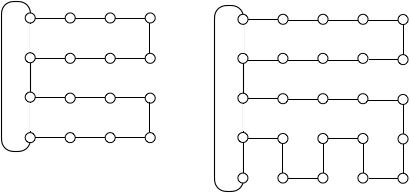
\includegraphics[scale=0.6]{FiguresGraph/HamiltonTorus}
       \caption{Principle for building hamiltonian cycles (even-even and odd-odd).}
  \label{fig:HamiltonTorus}
\end{center}
\end{figure}
\medskip

\noindent {\bf (d)}
One can craft a Hamiltonian cycle in $\q_n$ by
generating an {\it order-$n$ binary reflected Gray code}---so named
for its inventor, Bell Laboratories researcher \index{Gray, Frank}
Frank Gray; see \cite{PetersonW81}.  \index{Gray code} \index{binary
  reflected Gray code} Such a ``code'' is a cyclic enumeration of all
$2^n$ binary strings of length $n$ having the property that cyclically
adjacent \index{strings!cyclically adjacent} strings differ in only
one bit-position.  Length-$n$ strings $x_i$ and $x_j$ are {\it
  cyclically adjacent} in the Gray code $\langle x_0, \ x_1, \ldots,
x_{2^n-1} \rangle$ if $j = i+1 \bmod 2^n$.

\noindent
It is computationally easy to generate an order-$n$ Gray code from an
order-$(n-1)$ Gray code, as follows.

We note first that the order-$1$ code is the sequence $\langle 0, 1
\rangle$.

Inductively, to generate the order-$(k+1)$ Gray code from the
order-$k$ code:
\begin{itemize}
\item
Concatenate the order-$k$ code with a {\em reversed} copy of itself.
(It is the code-sequence that is reversed, not the individual strings.
For instance, as we go from the order-$2$ code $\langle x_0, \ x_1,
\ x_2, \ x_3 \rangle$ to the order-$3$ code, we concatenate that
sequence with $\langle x_3, \ x_2, \ x_1, \ x_0 \rangle$.)
\item
Augment each length-$k$ string in one copy of the order-$k$ Gray code
to length $(k+1)$ by prepending a $0$ to each string; and, augment
each length-$k$ string in the other (reversed) copy of the order-$k$
Gray code to length $(k+1)$ by prepending a $1$ to each string.
\end{itemize}
The following table illustrates the first few steps of this process.
\begin{equation}
\label{eq:gray-code}
 {\small
\begin{array}{|c|c|c|c|}
\hline
\mbox{Order } \ 1
  & \mbox{Order } \ 2
  & \mbox{Order } \ 3
  & \mbox{Order } \ 4 \\
\hline
0   & 00   & 000  &  0000 \\ 
1   & 01   & 001  &  0001 \\
    & 11   & 011  &  0011 \\
    & 10   & 010  &  0010 \\
    &      & 110  &  0110 \\
    &      & 111  &  0111 \\
    &      & 101  &  0101 \\
    &      & 100  &  0100 \\
    &      &      &  1100 \\  
    &      &      &  1101 \\  
    &      &      &  1111 \\  
    &      &      &  1110 \\  
    &      &      &  1010 \\  
    &      &      &  1011 \\  
    &      &      &  1001 \\  
    &      &      &  1000 \\  
\hline
\end{array} }
\end{equation}

We now sketch a proof that for each index $n \in \N^+$, the order-$n$
Gray code sequence specifies a Hamiltonian cycle in $\q_n$; exercises
will give the reader the opportunity to fill in details.  We verify
the following two assertions in turn:
\begin{enumerate}
\item
{\it The order-$n$ Gray code contains all $2^n$ length-$n$ binary
  strings.}
\item
{\it Every pair of cyclically adjacent strings in the order-$n$ Gray
  code differ in a single bit-position.}
\end{enumerate}

(1) We sketch the induction.  When $n=1$, the Gray code consists of
the two distinct strings $0$ and $1$.  Assume that the assertion holds
for $n=k$.  The order-$(k+1)$ code is obtained by taking two copies of
the order-$k$ code and prepending $0$ to the strings in one copy and
$1$ to the strings in the other copy.  The $2^k$ distinct binary
strings from the order-$k$ code thereby produce $2^{k+1}$ distinct
binary strings in the order-$(k+1)$ code.

(2) We distinguish three situations.  Let the adjacent strings be
string $x$, which appears in position $i$ of the code, and string $y$,
which appears in position $i+1 \bmod 2^n$ of the code.
  \begin{itemize}
  \item
Say that $i = 2^n-1$.  In this case $x$ is the last string in the
code, and $y$ is the first string.  By the ``refective'' nature of the
construction of the code, we know that $x = 1z$ and $y = 0z$ for some
length-$(n-1)$ binary string $z$.  Strings $x$ and $y$ therefore
differ in precisely one bit-position, namely, bit-position $0$.

  \item
Precisely the same argument shows that when $i = 2^{n-1} -1$, strings
$x$ and $y$ again differ precisely in bit-position $0$.

  \item
In all other cases, namely, when $i \in \{0,1, \ldots, 2^n-1\}
\setminus \{2^{n-1} -1, 2^n-1\}$, strings $x$ and $y$ share the same
first bit-position.  In fact, for some bit $\beta \in \{0,1\}$, $x =
\beta u$ and $y = \beta v$ for length-$(n-1)$ binary strings $u$ and
$v$ which are cyclically adjacent in the order-$(n-1)$ Gray code.  By
an inductive argument, $u$ and $v$ differ in precisely one
bit-position---which means that $x$ and $y$ also differ in precisely
one bit-position.
  \end{itemize}
  The previous analysis is summarized in Fig.~\ref{fig:HamiltonHypercude}.
  \begin{figure}[hbt]
\begin{center}
       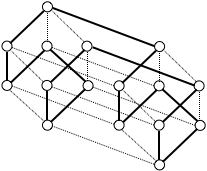
\includegraphics[scale=0.6]{FiguresGraph/HamiltonHypercube}
       \caption{Hamiltonian cycle in Hypercube using reflected Gray codes.}
  \label{fig:HamiltonHypercude}
\end{center}
\end{figure}


\noindent {\bf (e)}
By Proposition~\ref{thm:deBruin-linegraph}, each de Bruijn network
$\d_n$ is the line-digraph of the next bigger de Bruijn network,
$\d_{n+1}$.  Therefore, by definition of ``line (di)graph'', the fact
that $\d_n$ is (directed)-Eulerian
(Corollary~\ref{thm:deBruijn-Eulerian}) means that $\d_{n+1}$ is
(directed)-Hamiltonian.  \qed
\end{proof}


\subsubsection{Testing general graphs for Hamiltonianicity}
\label{sec:Hamiltonian-unweighted}

The techniques we use in Subsection~{\small\sf B} to investigate the
Hamiltonianicity of our ``named'' graphs exploit the detailed
structures of the individual graphs.  Thus, we cannot expect the proof
of Proposition~\ref{thm:named-graph-Hamiltonian} to suggest avenues
for determining whether an arbitrary given graph is Hamiltonian.  In
fact, quite sophisticated results proved in the early 1970s make a
strong mathematical argument that no set of case studies is likely to
have a major impact on the problem of testing general graphs for
Hamiltonianicity.  This is because, in common with the Satisfibility
problem {\sf 3SAT} of Section~\ref{sec:Satisfiability}, the
Hamiltonianicity-detection problem is {\sf NP}-complete.  We repeat
from our discussion in Section~\ref{sec:Satisfiability} that the
details of the theory of {\sf NP}-completeness are beyond the scope of
this text, but we do want the reader to recognize the following.
\begin{description}
\item
{\it The problem of deciding, given a graph $\g$ that is presented via
  a list of nodes and a list of edges, whether $\g$ admits a
  Hamiltonian path or a Hamiltonian cycle is {\sf NP}-complete.}
\end{description}


%%%%%%%%%%%%%%%%%%%%%%%%%%%%%%%%%%%

\section{$\oplus$ Pointers to Advanced Topics}
\label{sec:advanced-topics}

%**PROVIDE SOME REFERENCES

We conclude this chapter by mentioning a variety of topics that are
typically not covered---at least in depth---early in the curriculum,
but that are important enough that the reader should at least be aware
of them.  The topics we mention are motivated by virtually every
computational area that benefits from graph-theoretic models.  We have
tried to present each topic we touch on at a level of discourse that
will prepare the interested reader to delve more deeply into the
material, yet at a level of informality that will make the material
accessible to the more casual reader.  We thus strive for an intuitive
presentation that will not lead any reader astray.

The problem that we discuss in Section~\ref{sec:Relate-CS-Math-Probs}
illustrates how the {\em dynamic} models in the field of
algorithmics---``dynamic'' in the sense that they {\em do}
something---and the {\em structural} models provided by graph theory
can often provide beneficial illumination of one another.

Section~\ref{sec:graph-decompose} \index{graph!graph separators}
\index{graph!graph decomposition} focuses on the myriad computations
on graph that can be accomplished efficiently via recursive algorithms
that decompose, then reassemble, the graphs that they work on.

Section~\ref{sec:graph-evolve} \index{graph!evolving graphs}
introduces the increasingly important topic of graphs whose structure
changes dynamically over time.  One timely instance of this dynamic
evolution is the connectivity graph of the Internet.

Section~\ref{sec:hypergraphs} \index{graph!hypergraphs}
\index{hypergraphs} introduces {\it hypergraphs}, a generalization of
graphs that allows multi-entity relationships, in contrast to the
binary relationships mandated by graphs' two-element edges.
Hypergraph-based models find application in areas as diverse as:
\begin{itemize}
\item
{\it social networks:} Hyperedges can describe, e.g., collaboration
and collusion.
\item
{\it electronic networks:} Hyperedges can enable the design of
equi-potential nodes in voltage-driven technologies such as {\it
  VLSI}.
\item
{\it communication networks:} Hyperedges can model bus-oriented
communication.
\end{itemize}




\subsection{Relating Computational and Mathematical Problems}
\label{sec:Relate-CS-Math-Probs}

This 

\ignore{*******************

\subsubsection{The Route Inspection/ Chinese Postman Problem}
\label{sec:chinesePostman}

**HERE

After solving the preceding ``pure'' version of the Eulerian-tour
problem---which seeks a tour of a graph which crosses each edge
precisely once---we discuss an extension of this problem which allows
us to augment a graph $\g$ by adding multiple edges between the same
two nodes.  (Terminologically, we thereby convert $\g$ to a {\it
  multi-graph} \index{multi-graph} \index{graph!multi-graph}
consisting of nodes and {\it multi-edges}.) \index{multi-edge} Not
obviously, adding multi-edges can often convert a graph $\g$ that does
not admit an Eulerian cycle into a multi-graph that does admit an
Eulerian cycle.  The problem of finding the {\em smallest} such
augmentation of $\g$---i.e., of adding the fewest multi-edges---is
called the \index{Route Inspection Problem} {\it Route Inspection
  Problem}; it is also often called the {\it Chinese Postman Problem},
\index{Chinese Postman Problem} in honor of its inventor, the Chinese
mathematician Kwan Mei-Ko \index{Kwan Mei-Ko} \cite{Kwan60}.



This section is devoted to studying the {\it Route Inspection
  Problem}, \index{Route Inspection Problem} also known as the {\it
  Chinese Postman Problem}, \index{Chinese Postman Problem} in honor
of its inventor, the Chinese mathematician Kwan Mei-Ko \index{Kwan
  Mei-Ko} \cite{Kwan60}.  This problem seeks to add as few multi-edges
\index{graph!multi-graph!multi-edge} as possible to a graph $\g$ in
order to render $\g$ Eulerian.  (A {\it multi-graph} is ``almost'' an
undirected graph.  It differs from a true graph because of the
possible presence of multiple multi-edges that connect the same two
nodes.)

**HERE


We know from Proposition~\ref{thm:eulerian-cycle} that if all of
$\g$'s nodes have even node-degrees, then---{\em and only then}---$\g$
admits an Eulerian cycle.  Therefore, in this case, {\em zero}
multi-edges need be added to $\g$ to render it Eulerian.  

Let us now present the more general problem of determining a cycle that contains all the edges in any graph, in particular when
there exist some odd vertices. From the previous section, we know that there is no Eulerian cycle in this case and thus, 
any feasible solution should duplicate some edges.
The problem is to duplicate the minimum.
This problem is known as the {\it chinese postman} and it is described below (in a french equivalent version).

A postman moved recently from Grenoble to a small village in the country side. 
He asked himself how to organize his daily tour by bike for distributing the letters in the shortest possible time. 
The director of the post office gives him the map and 
fortunately, the postman had some old souvenir of previous lectures in Graph Theory.  
The tour starts from the post office and of course, the postman has to go through every roads for distributing the letters before coming back
to his office.
The underlying graph is $G=(V,E)$ where $V$ is the (finite) set of cross points and $E$ is the set of the links between the cross roads
weighted by the distances.  

Fig.~\ref{fig:EulerianInitial} presents an example of the chinese postman problem. 
\begin{figure}[hbt]
\begin{center}
       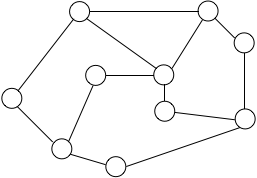
\includegraphics[scale=0.6]{FiguresGraph/EulerienInitial}
       \caption{An instance of the Chinese postman with $10$ cross-nodes.}
              \label{fig:EulerianInitial}
\end{center}
\end{figure}

\bigskip

This problem can be formulated mathematically in term of Eulerian
cycles.  Intuitively, the basic idea is to duplicate some edges that
are carefully chosen in order to use the previous construction of an
Eulerian tour of Section~\ref{sec:EulerianCycle} that will help the
postman to determine the optimal tour (of minimal length) using some
simple mathematical properties.
\bigskip

First, we know that there is an even number of odd vertices.
Considering the previous instance of the postman problem, there are $4$ such vertices (represented in grey in Fig.~\ref{fig:EulerianVodd}).

\begin{figure}[hbt]
\begin{center}
       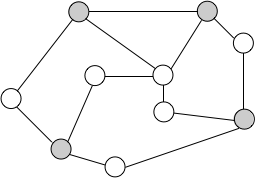
\includegraphics[scale=0.6]{FiguresGraph/EulerienVodd}
       \caption{The $4$ vertices with an odd degree in the previous instance.}
              \label{fig:EulerianVodd}
\end{center}
\end{figure}
\bigskip

As there exists a path between any pair of vertices of odd degree in $V_{odd}$,
we consider the complete graph whose vertices are the odd degree vertices weighting the edges with the shortest paths (denoted by $K_{odd}$).
As we mentioned in the preliminary properties, computing the shortest paths is a classical problem, which can be solved in polynomial time. 

\begin{figure}[hbt]
\begin{center}
       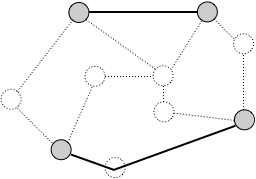
\includegraphics[scale=0.6]{FiguresGraph/EulerienPerfectMatching}
       \caption{The minimum weight perfect matching labelled by the shortest distances between the vertices of $V_{odd}$.}
              \label{fig:Eulerianperfectmatching}
\end{center}
\end{figure}
\bigskip

Then, it is possible to do the correspondence between the optimal solution of the postman problem and a perfect matching of minimal weight in $K_{odd}$
%Recall that a matching is a set of edges without common vertices. It is perfect if it has the maximum number of edges. 
by duplicating the edges of the minimal perfect matching.

\begin{figure}[hbt]
\begin{center}
       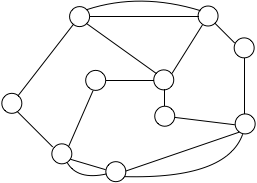
\includegraphics[scale=0.6]{FiguresGraph/EulerienFinal}
       \caption{Final step: adding the edges of the minimum perfect matching.}
              \label{fig:EulerianFinal}
\end{center}
\end{figure}

The main steps of the algorithm for determining the optimal tour are the following:

\begin{itemize}
\item Consider the complete graph with the odd vertices and compute its weight by the shortest paths.
Compute a perfect matching of minimal weight between these vertices. 
\item Duplicate all the edges along the paths of this matching.
\item Determine an Eulerian tour in this new graph with even degrees.
\end{itemize}

The optimality of this algorithm comes from the fact that the duplicated edges are the minimum possible ones.
% This is straightforward for two odd vertices.
Finally, all the vertices of the new graph are even since the degree of the odd vertices in $G$ is augmented by $1$
(extremities of the paths) and the other even vertices which are intermediate vertices of the paths remain even. 

\medskip

This short discussion is a good segu\'{e} to the material in the next
section, which leds valuable perspective on our brief study of
Hamiltonian paths and cycles---and, indeed, on the computational
implications of that work.
*************************}

\subsection{Graph Decomposition}
\label{sec:graph-decompose}
\index{graph!decomposition}
\index{graph!bisector}
\index{graph!separator}

The reader will certainly have noted that some ``named'' graphs are,
intuitively, more tightly interconnected than others.  From a purely
intellectual vantage point, it would be of interest to be able to
quantify the tightness of interconnection.  Among the various measures
that have been proposed, one stands out for its myriad algorithmic
implications: the notion of {\it graph separator}.  In fact, this
notion appears in the literature in several flavors.  An $n$-node,
$e$-edge graph $\g$ has:
\begin{itemize}
\item
an {\it $\alpha$-edge separator} of size $k$, 
\index{graph!$\alpha$-edge separator of size $k$} where $\alpha$ is a
real number with $\alpha \leq 1/2$ and $k$ is an integer with $k < n$,
precisely if:

\smallskip

one can partition $\g$ into two disjoint (not-necessarily connected)
subgraphs, each having $\leq \alpha n$ nodes, by removing $\leq k$
edges from $\g$.

\item
a {\it $\alpha$-node separator} of size $\ell$,
\index{graph!$\alpha$-node separator of size $\ell$}
where $\alpha$ is a real number with $\alpha \leq 1/2$ and $\ell$ is
an integer with $k < e$, precisely if:

\smallskip

one can partition $\g$ into two disjoint (not-necessarily connected)
subgraphs, each having $\leq \alpha n$ nodes, by removing $\leq \ell$
nodes from $\g$.
\end{itemize}
We replace the term ``separator'' with the term {\em ``bisector''} 
\index{graph!edge bisector} \index{graph!node bisector}
if both subgraphs after a separation operation have $\leq \lfloor
\frac{1}{2} n \rfloor$ nodes.

\medskip

Commonalities and differences in inherent separator sizes are often
not visually obvious.  For illustration, referring to the ``named''
graphs of Section~\ref{sec:graphs-important-families}:
\begin{itemize}
\item
It is certainly obvious that cycles are easier to bisect than cliques,
as measured by either edge or node bisectors.
\item
It is far less clear that de Bruijn networks and hypercubes are
roughly equal in ease to bisect, as measured by node bisectors.
\end{itemize}
But similar separation behavior has very important algorithmic
consequences.  For instance, the closeness in separation
characteristics between de Bruijn networks and hypercubes manifests
itself in a large range of algorithmic applications.  The range of
such applications is hinted at by sources that study the algorithmics
of laying out VLSI circuits (see, e.g., \cite{Leiserson85}) and
sources that study the ability of a network's interconnections to host
a range of communication patterns that enable efficient parallel
computation and communication (see, e.g.,
\cite{AnnexsteinBR90,Leiserson85,Ullman84}).


\medskip

There is a large literature that develops the algorithmics of finding
small separators for significant families of graphs.  An early star in
the firmament of such studies is the discovery in \cite{LiptonT79} of
a $1/3$-node separator of size $\sqrt{8n}$ for $n$-node planar graphs.
The dual problem of finding lower bounds on the sizes of graph
separators is a bit sparser but, of course, no less significant.  The
reader can find a comprehensive exposition on the theory of graph
separators in \cite{RosenbergH01}, including both the mathematics that
yields lower bounds on separator sizes and the algorithmics that
yields upper bounds.


\subsection{Graphs with Evolving Structure}
\label{sec:graph-evolve}
\index{graph!with evolving structure}

Classical problems in the area of graph algorithms will discuss
graphs, especially trees, whose structures evolve over time.  Such
evolution is observed, e.g., in the study of ``classical'' algorithmic
problems such as {\it Minimum Spanning Tree} and {\it Branch and
  Bound}; see, e.g., \cite{CLRS}.  What is certain to be more exciting
to the reader, though, are the ``modern'' topics where one encounters
graphs with evolving structure, such as {\it social networks} and {\it
  inter-networks} (e.g., the {\it Internet of Things}).

For ``classical'' topics, as exemplified by the two we have mentioned,
the mathematics covered in this chapter will provide the reader with
the background necessary to deal with graph evolution.  Indeed, this
evolution emerges as an inevitable concomitant of the algorithmics
that is superimposed upon the traditional structures of graph theory:
the challenge to the reader is to assimilate new algorithmic notions,
not new mathematics.

\index{graph!with evolving structure!social networks}
\index{graph!with evolving structure!inter-networks}
In contrast, the ``modern'' topics we have mentioned do require the
reader's assimilating new mathematics.  Dealing successfully with the
algorithmic issues that arise with social networks and inter-networks
requires the reader to understand the structures of the evolving
graph-oriented systems and how evolution changes these structures.
Among the interesting (and valuable) mathematical questions one can
pose is: When a new node applies to join an evolving network, which
node in the network is the best one to connect to, in order to best
facilitate one's interactions or influence within the community.  The
latter topic leads, e.g., to the study of {\em power-law} networks.
\index{graph!with evolving structure!social networks!power-law networks}
\index{graph!with power-law degreegrowth patterns}
\bigskip

\noindent \fbox{
\begin{minipage}{0.95\textwidth}
An evolving network is said to {\it obey a power law} if there exists
a real number $\gamma >0$ such that, for sufficiently large values of
the integer parameter $k$, the fraction of nodes in the network having
degree $k$ is proportional to $k^{-\gamma}$.
\end{minipage}
}
\bigskip

Little of the abstract work on power-law networks would likely be
studied in depth in any early course; indeed, the structure of these
networks is not yet well understood even in advanced settings.
Attempts to understand power laws with rigor have given rise to a
number of competing, rather sophisticated, abstract models---see,
e.g., \cite{AielloCL00,BarabasiA99,Bollobas85,ChenCGJSW}---and
numerous studies have attempted to understand the specific situations
wherein the abstract models reflect reality more or less
faithfully---see, e.g.,
\cite{BuT02,FaloutsosFF99,JaiswalRT04,TangmunarunkitGJSW02,ZeguraCD97}.


\subsection{Hypergraphs}
\label{sec:hypergraphs}
\index{graph!generalization to hypergraphs}
\index{hypergraph}

A large variety of modern computing-related topics benefit from the
structure inherent in graph-theoretic models but do not comfortably
conform to the {\em binary} relationships imposed by graphs' having
{\em two} nodes per edge.  A model that retains the structure of
graph-theoretic models without the binary constraint is the
generalization of graphs called {\em hypergraphs}.  A hypergraph has
nodes that play exactly the same role as with graphs, but in place of
a graph's binary edges, a hypergraph has {\em hyperedges}, each being
a set of nodes whose size is not restricted to $2$.  A rather general
treatment of hypergraphs can be found in the comprehensive
graph-theory text \cite{Berge73}; a specialized article that focuses
on some of the topics of this chapter, such as node-coloring, is
\cite{Lovasz73}.  Because of their inherent complexity, hypergraphs as
graph-theoretic objects are usually relegated to advanced courses.
However, the literature contains many studies of hypergraphs that are
``fine-tuned'' for specific computing-related application areas, and
many of these should be accessible without extensive mathematical
background.  Sample  computing-related application areas that benefit
from hypergraph-oriented models include the following.
\begin{itemize}
\item
Bus-connected parallel communication has been part of digital computer
\index{hypergraph!modeling bus-connected communication} design since
its earliest days.  The informal picture of such a system is that
there are communication channels that multiple agents can retrieve
message from and post messages to.  In hypergraph-oriented terms: the
nodes/communicating agents aggregate into groups/hyperedges.  Each
group's agents share ``read/write'' access to a specific channel.  A
specialized genre of hypergraph that was invented to study the
described scenario is the {\it interval hypergraph}
\index{hypergraph!interval hyergraph} model developed in
\cite{Rosenberg89a}.

\item
Modern electronic circuits are implemented using integrated circuit
\index{hypergraph!modeling integrated circuits} technology,
specifically, {\em VLSI: Very Large Scale Integrated circuitry}; see,
e.g., \cite{Mead-Conway}.  These technologies tend to be
voltage-driven, rather than current-driven.  Accordingly, much of the
attention when designing circuits centers on the coordination of
equi-potential points in a network, rather than on point-to-point
transmission of signals.  Hypercubes are tailor-made for such
technologies.  A crucially important issue that arises because of the
design strengths and weaknesses of  VLSI technology is {\it fault
  tolerance}---how to cope with the inevitable faulty transistors in
massive VLSI systems.  Even mathematically quite-accessible ideas can
provide provocative ideas about this important topics; see, e.g.,
\cite{Rosenberg85a}

\item
Social networks have become so prevalent in society that no one will
be surprised to learn that many approaches to modeling the networks'
interconnectivity have been studied.  In
Section~\ref{sec:graph-evolve}, we discussed an interconnectivity
model based on evolving graphs and clustering within such graphs.
More recently, hypergraph-based models
\index{hypergraph!modeling interconnectivity in social networks}
have also been proposed; see, e.g., \cite{Amatoetal17,LiuBV10}.
\end{itemize}





